%!TEX program = xelatex
% 完整编译: xelatex -> biber/bibtex -> xelatex -> xelatex
\documentclass[lang=cn,11pt,a4paper]{elegantpaper}
\usepackage{setspace}
\usepackage{titlesec}
\usepackage{titling}
\usepackage{caption}
\usepackage{comment}

\begin{comment}
% 设置标题格式
\titleformat{\section}{\normalfont\fontsize{12}{15}\bfseries}{\thesection}{1em}{}
\titleformat{\subsection}{\normalfont\fontsize{12}{15}\bfseries}{\thesubsection}{1em}{}
\titlespacing{\section}{0pt}{*4}{*1.5}
\titlespacing{\subsection}{0pt}{*4}{*1.5}
%%%%%%
\end{comment}

% 设置标题信息

\title{\textbf{\Huge 地基雷达探测飞机研究分析}\vfill}

\author{林思宇\ \ 徐炜航\ \ 刘赫楠\\陈梓萌\ \ \ 黄子阳}

\date{\zhtoday}


% 本文档命令
\usepackage{array}
\newcommand{\ccr}[1]{\makecell{{\color{#1}\rule{1cm}{1cm}}}}

\begin{document}

\setcounter{secnumdepth}{4}
\setcounter{tocdepth}{4}

\maketitle

\newpage
\begin{abstract}
本文为 \href{https://github.com/ElegantLaTeX/ElegantPaper/}{ElegantPaper} 的说明文档。此模板基于 \LaTeX{} 的 article 类,专为工作论文写作而设计。设计这个模板的初衷是让作者不用关心工作论文的格式,专心写作,从而有更加舒心的写作体验。如果你有其他问题、建议或者报告 bug,可以在 \href{https://github.com/ElegantLaTeX/ElegantPaper/issues}{GitHub::ElegantPaper/issues} 留言。如果你想了解更多 Elegant\LaTeX{} 项目组设计的模板,请访问 \href{https://github.com/ElegantLaTeX/}{GitHub::ElegantLaTeX}。
\keywords{Elegant\LaTeX{},工作论文,模板}
\end{abstract}
\thispagestyle{empty}
\newpage
\tableofcontents
\thispagestyle{empty}
\newpage
\setcounter{page}{1}

\section{信号的发送}
\input{信号的发生与发送/调制发送}


\section{信号接收与处理}
\input{信号预处理/信号预处理}
\input{目标检测/目标检测}
\input{目标参数的估计及成像处理/目标参数的估计及成像处理}
\pagestyle{plain}

\subsection{\textbf{目标追踪}}
\subsubsection{卡尔曼滤波}
\paragraph{卡尔曼滤波的基本原理}~{}

        卡尔曼滤波算法是指通过上一时刻的状态数据的估计值对当前的观测值进行修正和更新,采用“预测-实测-修正”的计算方式求得数据的最优预测值。在数据的处理过程中,它可以对数据中的噪声起到一定的抑制作用,实现对目标当前运动状态数据的平滑处理和将来运动状态的估计预测,数据的更新过程是依据目标的状态方程进行更新,主要包括对状态变量和量测数据的更新,状态变量X的更新方程为:
    
                 \begin{center}
                     $\begin{array}{r}\boldsymbol{X}(k)=\boldsymbol{F} \boldsymbol{X}(k-1)+\boldsymbol{G} V(k-1) \\P(k)=\boldsymbol{F} P(k-1) \boldsymbol{F}^{\mathrm{T}}+Q\end{array}$
                 \end{center}
                 
\begin{flushleft}
式中,$F$为状态矩阵;$Q$为数据噪声;$P(k)$为协方差。测量数值的更新方程为:
\end{flushleft}

                \begin{center}
                    $\begin{array}{c}K(k)=P(k) \boldsymbol{H}^{\mathrm{T}} \boldsymbol{H}\left(\boldsymbol{H} P(k) \boldsymbol{H}^{\mathrm{T}}+W\right)^{-1} \\\boldsymbol{X}(k+1)=\boldsymbol{X}(k)+k(Z(k)-\boldsymbol{X}(k) \boldsymbol{H}) \\P(k+1)=(\boldsymbol{I}-k \boldsymbol{H}) P(k)\end{array}$        
                \end{center}
                
\begin{flushleft}
    式中,$K(k)$ 为卡尔曼增益;$Z(k)$为观测数据;$\boldsymbol{H}$ 为观测矩阵;$W$为噪声; $\boldsymbol{I}$ 为单位矩阵。
\end{flushleft}
\paragraph{卡尔曼滤波的特性}~{}


    卡尔曼滤波具有如下的特性:
    \begin{enumerate}[(1)]
        \item 卡尔曼滤波算法不仅适用于平稳序列的滤波,而且适用于非平稳或平稳马尔可夫序列或高斯——马尔可夫序列的滤波,因此应用范围十分广泛。 
        \item 由于卡尔曼滤波的基本方程是时间域内的递推形式,其计算过程是一个不断地“预测-修正”过程,在求解时不要求存储大量的数据,并且一旦观测到了新的数据,随时可以算得新的滤波值,因此这种滤波方法非常便于实时处理。
        \item 增益矩阵与观测值无关,可以预先算出;增益矩阵与观测噪声方差阵$D_{\Delta}(k)$ 成反比,即当观测噪声增大时,滤波增益应取小一些,以减弱观测噪声对滤波值的影响;与系统动态噪声方差阵 $D_{\Omega}(k)$ 成正比。即当系统噪声变小时,增益矩阵应小些以便给与较小的修正。
        \item $D_{X}(k / k)$  是所有估计的最小方差阵。
    \end{enumerate}


\paragraph{卡尔曼滤波的不足}~{}

        卡尔曼滤波中的状态方程,常用数学模型来描述一个物理问题,这种陈述常受到对客观物理现象的了解和数学表达程度的局限而产生模型误差。观测方程的表达式要求是线性形式,而实际的观测量和状态参数间大都是非线性函数,非线性二次以上高次项的舍去,以及观测粗差等原因,也将使观测方程产生模型误差。
        
        理想情况下,卡尔曼滤波是线性无偏最小方差估计,根据滤波稳定性原理,对于一致完全可控和一致完全可观测系统,随着时间的推移,观测数据的增多,滤波估计的精度应该越来越高,滤波误差方差阵或者趋于稳态值,或者有界。但是在实际应用中,由滤波得到的状态估计可能是有偏的,且估计误差的方差也可能很大,远远超出了按计算公式计算的方差所定出的范围,更有甚者,其滤波误差的均值与方差都有可能趋于无穷大,这种现象,在滤波理论中称为滤波的发散现象。显然当滤波发散时,就完全失去了滤波的最优作用。因此在实际应用中,必须抑制这种现象。 
        
        导致最优滤波发散的原因主要有以下几种:
        \begin{enumerate}[(1)]
            \item 描述系统特性的数学模型和噪声模型的统计模型不准确,不能真实地反映物体过程,使模型与获得的观测值不匹配,导致滤波发散。
            \item 观测方程表达式是线性,而实际观测量与状态参数之间大都是非线性函数,非线性二次以上的高次项舍去,以及观测粗差等原因,导致模型存在误差,可能会导致发散。
            \item 卡尔曼滤波理论对动态系统提出了严格的要求,即要求系统噪声和观测噪声为零均值白噪声。这一条件在实践中难以满足,导致卡尔曼滤波产生发散现象,从而使状态估计不可信。可见动态噪声和观测噪声的方差和协方差估计是引起发散现象的重要因素。
            \item 卡尔曼滤波是递推过程,随着滤波步数的增加,舍入误差逐渐积累,如果计算机步长有限,这种积累有可能使估计的误差方差阵失去非负定性甚至失去对称性,使增益矩阵的计算值逐渐失去合适的加权作用而导致发散。
        \end{enumerate}
        
        应该指出,以上各种原因也不一定会引起滤波发散,视具体情况而定。

\subsubsection{粒子滤波}

\paragraph{地波雷达的多种探测方法}~{}

        高频地波雷达(High Freguency Surface Wave Radar, HFSWR)是大范围海上船只目标监视监测的主要手段,它利用高频电磁波(3~30MHz)沿海面爬行来实现超视距的目标(船只、低空飞机等)探测,可以实时提供运动目标的位置和航速航向等信息,探测距离最远可达300km,因此它又被称地波超视距雷达。
        
        传统的高频地波雷达目标探测方法采用的是先检测后跟踪(Detect-Before-Track,DBT)的思想,该方法对于回波能量较弱、信噪比较低的目标单时刻的检测效果不佳,从而使得连续时刻的目标跟踪性能下降。
        
        检测与跟踪联合处理方法可以解决弱目标检测困难的问题,其思路是:对单帧雷达回波数据不进行目标有无判断,而是利用目标在时空上的关联特性和杂波噪声的随机性,进行多帧数据累积,从而实现同一目标的回波能量累积,由此提高目标信噪比,完成目标的检测判决和航迹跟踪。检测与跟踪联合处理方法由于不设置检测门限,能充分利用目标回波谱的原始信息,即可减少先检测后跟踪过程中的点迹与航迹关联问题,亦可降低算法复杂度。
       
        目前,国内外已发展了多种检测前跟踪(Track-Before-Detect,TBD)方法,均可被用于实现地波雷达目标检测与跟踪联合处理。主要方法有:动态规划(Dynamic Programming,DP)法、粒子滤波(Particle Filter,PF)法和三维匹配滤波(3-D Matched Filters)法等。
        
\paragraph{ 粒子滤波法的优势}~{}

        粒子滤波法将目标航迹跟踪问题转换为目标的概率密度函数估计问题,相对于动态规划、三维匹配滤波等方法,它具有估计的目标状态在理论上最优的特点,适合于类似地波雷达这种非线性、非高斯的系统,且因其递归结构特点算法容易实现。
        
\paragraph{粒子滤波法原理}~{}

        在粒子滤波法中,通过使用序贯重要性采样方法对目标状态进行采样,得到一组带有权值的随机样本即“粒子” $\left\{x_{1: k}^{i}, w_{k}^{i}\right\}_{i=1}^{N}$ ,当采样的样本集足够大的时候,经过重要性采样获得的这组随机粒子就可以用来描述目标的后验概率密度函数   $p\left(x_{1: k} \mid Z_{1: k}\right)\left(x_{1: k}=\left\{x_{j} \mid j=1,2, \cdots, k\right\}\right.  $ 表示目标的状态序列,  $Z_{1: k}=\left\{z_{1}, z_{2}, \cdots\right. ,  \left.z_{k}\right\}  $ 表示目标的量测值序列, l 为似然比, k 为自然数)。一般在经过多次迭代后,粒子会出现退化现象,因此,在重要性采样结束后,还需要对粒子进行重采样。最终目标状态的后验概率密度可表示为 
      \begin{center}
           $p\left(x_{1, k} \mid Z_{1, k}\right) \approx \sum_{i=1}^{N} w_{k}^{i} \delta\left(x_{1, k}-x_{1, k}^{i}\right),$
      \end{center}
  \begin{flushleft}
    式中,$i$ 为自然数。
\end{flushleft}

        粒子滤波的粒子权重既可以构造检测似然比以实现目标检测,又可以通过粒子权重与粒子状态的加权估计目标的状态,从而实现目标的检测与跟踪联合处理。粒子权重与检测似然比之间的关系为
     \begin{center}
           $L_{k}=\frac{p\left(Z_{k} \mid H_{1}\right)}{p\left(Z_{k} \mid H_{0}\right)} \approx \prod_{\substack{i \in C_{i}\left(x_{k}\right) \\ j \in C_{j}\left(x_{k}\right)}} l\left(z_{k}^{(i, j)} \mid x_{k}\right)=\frac{1}{N} \sum_{i=1}^{N} w_{k}^{i},$
     \end{center}
 \begin{flushleft}
      式中,  $L_{k}$  为目标k时刻的似然比;  $H_{1}$  为目标存在;  $H_{0}$  为目标不存在;  $p\left(z_{k} \mid H_{1}\right)$  为目标存在时的概率密度;  $p\left(z_{k} \mid H_{0}\right)$  为目标不存在时的概率密度;  $C_{i}$  和  $C_{j}$  为受目标影响的单元; 则目标k时刻的递归似然比计算公式为  $\Lambda_{k} \approx \Lambda_{k-1} \prod_{\substack{i \in C_{i}\left(x_{k}\right) \\ j \in C_{j}\left(x_{k}\right)}} l\left(z_{k}^{(i, j)} \mid x_{k}\right) \approx \Lambda_{k-1} \frac{1}{N} \sum_{i=1}^{N} w_{k}^{i}$  。
 \end{flushleft}
 
        将计算得到的目标似然比与设定的阈值进行比较,判断目标是否存在。若目标存在,则在完成粒子重采样后按照公式 $x_{k}=\sum_{i=1}^{N} w_{k}^{i} \hat{x}_{k}^{i}$ 进行目标的状态估计。


\section{雷达系统优化}
\input{优化/优化}












\section{模板使用须知}

\subsection{注意事项}

时隔两年,本模板迎来更新,中间发生了很多变化,两个主要变化是参考文献与字体设定,\textbf{使用前请务必仔细阅读本文档}。

\textbf{文献部分}:我们将 bibtex 的默认文献编译方式改为 biblatex,不过我们也提供了两个后端,\lstinline{bibend=biber} 和 \lstinline{bibend=bibtex}。特别需要注意的是,从 0.10 开始,文献文件改为 \lstinline{reference.bib},与 ElegantBook 保持一致,而参考文献的引文样式等更多格式,请参考后文参考文献部分,更多样式可以参考 biblatex 文档。 

\textbf{字体部分},我们将 newtxtext 宏包的支持方式改为了字体名称设定方式,设定英文字体为 TeX Gyre Terms/Heros,,英文字体部分,根据编译方式选择不同字体。对于一般用户而言,不太需要关心这部分内容。

另外,中文请务必使用 \hologo{XeLaTeX} 编译。

\subsection{模板介绍}

此模板基于 \LaTeX{} 的标准文类 article 设计,所以 article 文类的选项也能传递给本模板,比如 \lstinline{a4paper, 11pt} 等等。

\begin{lstlisting}
\documentclass[a4paper,11pt]{elegantpaper}
\end{lstlisting}

\textbf{注意}:Elegant\LaTeX{} 系列模板已经全部上传至 \href{https://www.overleaf.com/latex/templates/elegantpaper-template/yzghrqjhmmmr}{Overleaf} 上,用户可以在线使用。另外,为了方便国内用户,模板也已经传至\href{https://gitee.com/ElegantLaTeX/ElegantPaper}{码云}。


\subsection{全局选项}
此模板定义了一个语言选项 \lstinline{lang},可以选择英文模式 \lstinline{lang=en}(默认)或者中文模式 \lstinline{lang=cn}。当选择中文模式时,图表的标题引导词以及参考文献,定理引导词等信息会变成中文。你可以通过下面两种方式来选择语言模式:
\begin{lstlisting}
\documentclass[lang=cn]{elegantpaper} % or
\documentclass{cn}{elegantpaper} 
\end{lstlisting}

\textbf{注意:} 英文模式下,由于没有添加中文宏包,无法输入中文。如果需要输入中文,可以通过在导言区引入中文宏包 \lstinline{ctex} 或者加入 \lstinline{xeCJK} 宏包后自行设置字体。 
\begin{lstlisting}
\usepackage[UTF8,scheme=plain]{ctex}
\end{lstlisting}

\subsection{数学字体选项}

本模板定义了一个数学字体选项(\lstinline{math}),可选项有三个:
\begin{enumerate}
  \item \lstinline{math=cm}(默认),使用 \LaTeX{} 默认数学字体(推荐,无需声明);
  \item \lstinline{math=newtx},使用 \lstinline{newtxmath} 设置数学字体(潜在问题比较多)。
  \item \lstinline{math=mtpro2},使用 \lstinline{mtpro2} 宏包设置数学字体,要求用户已经成功安装此宏包。
\end{enumerate}

\subsection{中文字体选项}

模板提供中文字体选项 \lstinline{chinesefont},可选项有
\begin{enumerate}
  \item \lstinline{ctexfont}:默认选项,使用 \lstinline{ctex} 宏包根据系统自行选择字体,可能存在字体缺失的问题,更多内容参考 \lstinline{ctex} 宏包\href{https://ctan.org/pkg/ctex}{官方文档}\footnote{可以使用命令提示符,输入 \lstinline{texdoc ctex} 调出本地 \lstinline{ctex} 宏包文档}。
  \item \lstinline{founder}:方正字体选项(\textbf{需要安装方正字体}),后台调用 \lstinline{ctex} 宏包并且使用 \lstinline{fontset=none} 选项,然后设置字体为方正四款免费字体,方正字体下载注意事项见后文,用户只需要安装方正字体即可使用该选项。
  \item \lstinline{nofont}:后台会调用 \lstinline{ctex} 宏包并且使用 \lstinline{fontset=none} 选项,不设定中文字体,用户可以自行设置中文字体,具体见后文。
\end{enumerate}

\subsubsection{方正字体选项}
由于使用 \lstinline{ctex} 宏包默认调用系统已有的字体,部分系统字体缺失严重,因此,用户希望能够使用其它字体,我们推荐使用方正字体。方正的{\songti 方正书宋}、{\heiti 方正黑体}、{\kaishu 方正楷体}、{\fangsong 方正仿宋}四款字体均可免费试用,且可用于商业用途。用户可以自行从\href{http://www.foundertype.com/}{方正字体官网}下载此四款字体,在下载的时候请\textbf{务必}注意选择 GBK 字符集,也可以使用 \href{https://www.latexstudio.net/}{\LaTeX{} 工作室}提供的\href{https://pan.baidu.com/s/1BgbQM7LoinY7m8yeP25Y7Q}{方正字体,提取码为:njy9} 进行安装。安装时,{\kaishu Win 10 用户请右键选择为全部用户安装,否则会找不到字体。}

\begin{figure}[!htb]
\centering
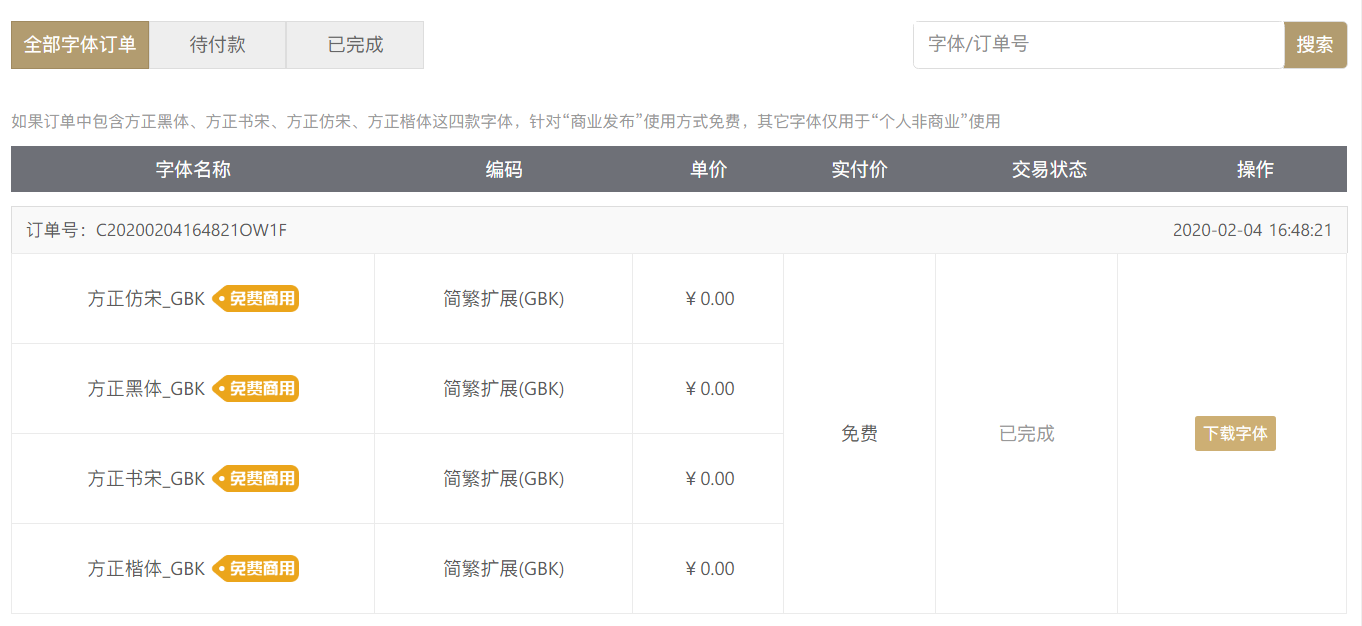
\includegraphics[width=0.9\textwidth]{founder.png}
\end{figure}

\subsubsection{其他中文字体}
如果你想完全自定义字体\footnote{这里仍然以方正字体为例。},你可以选择 \lstinline{chinesefont=nofont},然后在导言区设置即可,可以参考下方代码:
\begin{lstlisting}
\setCJKmainfont[BoldFont={FZHei-B01},ItalicFont={FZKai-Z03}]{FZShuSong-Z01}
\setCJKsansfont[BoldFont={FZHei-B01}]{FZKai-Z03}
\setCJKmonofont[BoldFont={FZHei-B01}]{FZFangSong-Z02}
\setCJKfamilyfont{zhsong}{FZShuSong-Z01}
\setCJKfamilyfont{zhhei}{FZHei-B01}
\setCJKfamilyfont{zhkai}[BoldFont={FZHei-B01}]{FZKai-Z03}
\setCJKfamilyfont{zhfs}[BoldFont={FZHei-B01}]{FZFangSong-Z02}
\newcommand*{\songti}{\CJKfamily{zhsong}}
\newcommand*{\heiti}{\CJKfamily{zhhei}}
\newcommand*{\kaishu}{\CJKfamily{zhkai}}
\newcommand*{\fangsong}{\CJKfamily{zhfs}}
\end{lstlisting}



\subsection{自定义命令}
此模板并没有修改任何默认的 \LaTeX{} 命令或者环境\footnote{目的是保证代码的可复用性,请用户关注内容,不要太在意格式,这才是本工作论文模板的意义。}。另外,我自定义了 4 个命令:
\begin{enumerate}
  \item \lstinline{\email}:创建邮箱地址的链接,比如 \email{ddswhu@outlook.com};
  \item \lstinline{\figref}:用法和 \lstinline{\ref} 类似,但是会在插图的标题前添加 <\textbf{图 n}> ;
  \item \lstinline{\tabref}:用法和 \lstinline{\ref} 类似,但是会在表格的标题前添加 <\textbf{表 n}>;
  \item \lstinline{\keywords}:为摘要环境添加关键词。
\end{enumerate}

\subsection{参考文献}

文献部分,本模板调用了 biblatex 宏包,并提供了 biber(默认) 和 bibtex 两个后端选项,可以使用 \lstinline{bibend} 进行修改:

\begin{lstlisting}
  \documentclass[bibtex]{elegantpaper}
  \documentclass[bibend=bibtex]{elegantpaper}
\end{lstlisting}

关于文献条目(bib item),你可以在谷歌学术,Mendeley,Endnote 中取,然后把它们添加到 \lstinline{reference.bib} 中。在文中引用的时候,引用它们的键值(bib key)即可。

为了方便文献样式修改,模板引入了 \lstinline{bibstyle} 和 \lstinline{citestyle} 选项,默认均为数字格式(numeric),参考文献示例:\cite{cn1,en2,en3} 使用了中国一个大型的 P2P 平台(人人贷)的数据来检验男性投资者和女性投资者在投资表现上是否有显著差异。

如果需要设置为国标 GB7714-2015,需要使用:
\begin{lstlisting}
  \documentclass[citestyle=gb7714-2015, bibstyle=gb7714-2015]{elegantpaper} 
\end{lstlisting}

如果需要添加排序方式,可以在导言区加入
\begin{lstlisting}
  \ExecuteBibliographyOptions{sorting=ynt}
\end{lstlisting}

启用国标之后,可以加入 \lstinline{sorting=gb7714-2015}。


\section{使用 newtx 系列字体}

如果需要使用原先版本的 \lstinline{newtx} 系列字体,可以通过显示声明数学字体:

\begin{lstlisting}
\documentclass[math=newtx]{elegantpaper}
\end{lstlisting}

\subsection{连字符}

如果使用 \lstinline{newtx} 系列字体宏包,需要注意下连字符的问题。
\begin{equation}
  \int_{R^q} f(x,y) dy.\emph{of\kern0pt f}
\end{equation}

\begin{lstlisting}
\begin{equation}
  \int_{R^q} f(x,y) dy.\emph{of \kern0pt f}
\end{equation}
\end{lstlisting}

\subsection{宏包冲突}

有用户反馈模板在使用 \lstinline{yhmath} 以及 \lstinline{esvect} 等宏包时会报错:
\begin{lstlisting}
LaTeX Error:
   Too many symbol fonts declared.
\end{lstlisting}

原因是在使用 \lstinline{newtxmath} 宏包时,重新定义了数学字体用于大型操作符,达到了 {\heiti 最多 16 个数学字体} 的上限,在调用其他宏包的时候,无法新增数学字体。为了减少调用非常用宏包,在此给出如何调用 \lstinline{yhmath} 以及 \lstinline{esvect} 宏包的方法。

请在 \lstinline{elegantpaper.cls} 内搜索 \lstinline{yhmath} 或者 \lstinline{esvect},将你所需要的宏包加载语句\textit{取消注释}即可。


\section{常见问题 FAQ}

\begin{enumerate}[label=\arabic*).]
  \item \textit{如何删除版本信息?}\\
    导言区不写 \lstinline|\version{x.xx}| 即可。
  \item \textit{如何删除日期?}\\
    需要注意的是,与版本 \lstinline{\version} 不同的是,导言区不写或注释 \lstinline{\date} 的话,仍然会打印出当日日期,原因是 \lstinline{\date} 有默认参数。如果不需要日期的话,日期可以留空即可,也即 \lstinline|\date{}|。
  \item \textit{如何获得中文日期?}\\
    为了获得中文日期,必须在中文模式下\footnote{英文模式下,由于未加载中文宏包,无法输入中文。},使用 \lstinline|\date{\zhdate{2019/10/11}}|,如果需要当天的汉化日期,可以使用 \lstinline|\date{\zhtoday}|,这两个命令都来源于 \href{https://ctan.org/pkg/zhnumber}{\lstinline{zhnumber}} 宏包。
  \item \textit{如何添加多个作者?}\\
    在 \lstinline{\author} 里面使用 \lstinline{\and},作者单位可以用 \lstinline{\\} 换行。
    \begin{lstlisting}
    \author{author 1\\ org. 1 \and author 2 \\ org. 2 }
    \end{lstlisting}
  \item \textit{如何添加中英文摘要?}\\
    请参考 \href{https://github.com/ElegantLaTeX/ElegantPaper/issues/5}{GitHub::ElegantPaper/issues/5}
\end{enumerate}


\section{致谢}

特别感谢 \href{https://github.com/sikouhjw}{sikouhjw} 和 \href{https://github.com/syvshc}{syvshc}  长期以来对于 Github 上 issue 的快速回应,以及各个社区论坛对于 ElegantLaTeX 相关问题的回复。特别感谢 ChinaTeX 以及 \href{http://www.latexstudio.net/}{LaTeX 工作室} 对于本系列模板的大力宣传与推广。

如果你喜欢我们的模板,你可以在 Github 上收藏我们的模板。





\newpage
\pagestyle{plain}
\setcounter{page}{7}
\nocite{*}
\printbibliography[heading=bibintoc, title=\ebibname]
\appendix
%\appendixpage
\addappheadtotoc

\end{document}

